\documentclass[twocolumn]{article}

\usepackage[utf8]{inputenc}
\usepackage[T1]{fontenc}
\usepackage[margin=1.25in]{geometry}
\usepackage{authblk}
\usepackage{setspace}
\usepackage{graphicx}
\graphicspath{{./img/}}
\usepackage{amsmath}
\usepackage{booktabs}
\usepackage{hyperref}
\usepackage{float}

\setlength{\columnsep}{24pt}
\setstretch{1.15}

\title{Unsupervised Text Clustering with K-means}

\author{Cesare Fraccaroli - VR533061}

\affil{NLP Course Project}

\date{}

\begin{document}
\twocolumn[
\begin{@twocolumnfalse}

\maketitle

\begin{abstract}
Three document embeddings are compared: \textbf{custom TF-IDF} (from scratch), \textbf{scikit-learn TF-IDF}, and \textbf{Gensim Word2Vec}, for \textbf{K-Means} on \textit{Reuters}. Preprocessing and clustering are decoupled via CSV so stages can be re-run separately; tokenization, stopwords, stemming, and embedding are configurable flags. \textbf{Word2Vec} gives the best numbers (Silhouette 0.31, Davies-Bouldin 1.39). TF-IDF only gives usable clusters after TruncatedSVD.
\end{abstract}
\vspace{1em}
\end{@twocolumnfalse}
]

% =================================================================
\section{Introduction}
% =================================================================

We look at how text representation choice affects \textbf{K-Means} on \textit{Reuters-21578} (10,788 documents, 90 categories). Documents are \textit{multi-labeled} (mean 1.24 categories each) and the distribution is \textit{heavily imbalanced}: \textit{earn} and \textit{acq} have 3,000+ documents each. That makes unsupervised partitioning non-trivial.

% =================================================================
\section{Design Choices}
% =================================================================

\subsection{Pipeline Architecture}

The pipeline has two stages: preprocessing (run once) and clustering (re-run as needed).

\begin{enumerate}
    \item \textbf{Preprocessing} (\texttt{preprocess.py}): raw text $\rightarrow$ NLP steps $\rightarrow$ embedding $\rightarrow$ optional SVD $\rightarrow$ vectors saved as CSV.
    \item \textbf{Clustering} (\texttt{cluster.py}, \texttt{tune.py}): load CSV $\rightarrow$ K-Means $\rightarrow$ evaluation.
\end{enumerate}

Vectors are written to CSV, so clustering can be re-run for different $k$ or distances without recomputing embeddings. Split is \textbf{80/20} (train 8,631; test 2,157), fixed seed.

\subsection{Configurable Preprocessing}

Flags switch each step on or off:

\begin{itemize}
    \item \texttt{--tokenize}: Penn Treebank tokenization via NLTK \texttt{word\_tokenize}. Required for all embeddings.
    \item \texttt{--stopwords}: removes 179 English stopwords (NLTK corpus).
    \item \texttt{--stem}: Porter Stemmer collapses morphological variants (\textit{running}, \textit{runs}, \textit{ran} $\rightarrow$ \textit{run}) and shrinks vocabulary. We preferred stemming over lemmatization for speed and simplicity; the downside is occasional over-stemming.
\end{itemize}

Preprocessing can be ablated without code changes.

\subsection{Embedding Methods}

The \texttt{--embedding} flag selects one of three strategies:

\begin{table}[H]
\centering
\small
\begin{tabular}{lrl}
\toprule
\textbf{Embedding} & \textbf{Dims} & \textbf{Key property} \\
\midrule
\texttt{tfidf-custom}   & $\sim$39k & Sparse, from-scratch impl. \\
\texttt{tfidf-sklearn}  & $\sim$21k & Sparse, built-in norms \\
\texttt{word2vec}        & 100       & Dense, semantic \\
\bottomrule
\end{tabular}
\label{tab:embeddings}
\end{table}

\begin{align*}
    \mathrm{TF}(w, d)      &= \frac{\mathrm{count}(w, d)}{|d|} \\
    \mathrm{IDF}(w)        &= \log\left(\frac{N}{\mathrm{df}(w)}\right) \\
    \mathrm{TF\text{-}IDF}(w, d) &= \mathrm{TF}(w, d) \times \mathrm{IDF}(w)
\end{align*}
where $w$ is a word, $d$ is a document, $N$ is the total number of documents, and $\mathrm{df}(w)$ is the number of documents containing $w$.

Both TF-IDF variants give \textit{high-dimensional sparse} vectors (most entries zero). Vocabulary size differs ($\sim$39k vs.\ $\sim$21k) because of scikit-learn's tokenization. \textbf{Word2Vec} instead uses the \textbf{L2}-normalized mean of word vectors: \textit{dense}, fixed size, \textit{semantic similarity} rather than \textit{lexical overlap}.

\subsection{Dimensionality Reduction (SVD)}

In 20k to 39k dimensions, TF-IDF vectors hit the \textit{curse of dimensionality}: pairwise \textbf{cosine distances} tend to look alike, and K-Means struggles. \textbf{TruncatedSVD} (same idea as \textit{Latent Semantic Analysis}) reduces them to 300 components, keeping most of the useful variance and dropping noise from rare terms.

SVD is applied at preprocessing (\texttt{--svd 300}), fit on the \textit{training set} and applied to both splits so clustering and evaluation use the same \textit{vector space}. Applying SVD only inside the clusterer would leave evaluation in the original space and skew the metrics.

Word2Vec is already 100 \textit{dense} dimensions; no SVD.

\subsection{Clustering and $k$ Selection}

Clustering: NLTK \texttt{KMeansClusterer}, \textbf{cosine distance}, \textbf{L2} norm. $k$ is chosen by the \textbf{elbow method}: \textbf{WCSS} vs $k$, pick the bend where adding clusters hardly helps.

% =================================================================
\section{Results}
% =================================================================

\subsection{Elbow Analysis}

WCSS for $k = 1$ to $10$ (Figures~\ref{fig:elbow_custom} to \ref{fig:elbow_w2v}).

\begin{figure}[H]
\centering
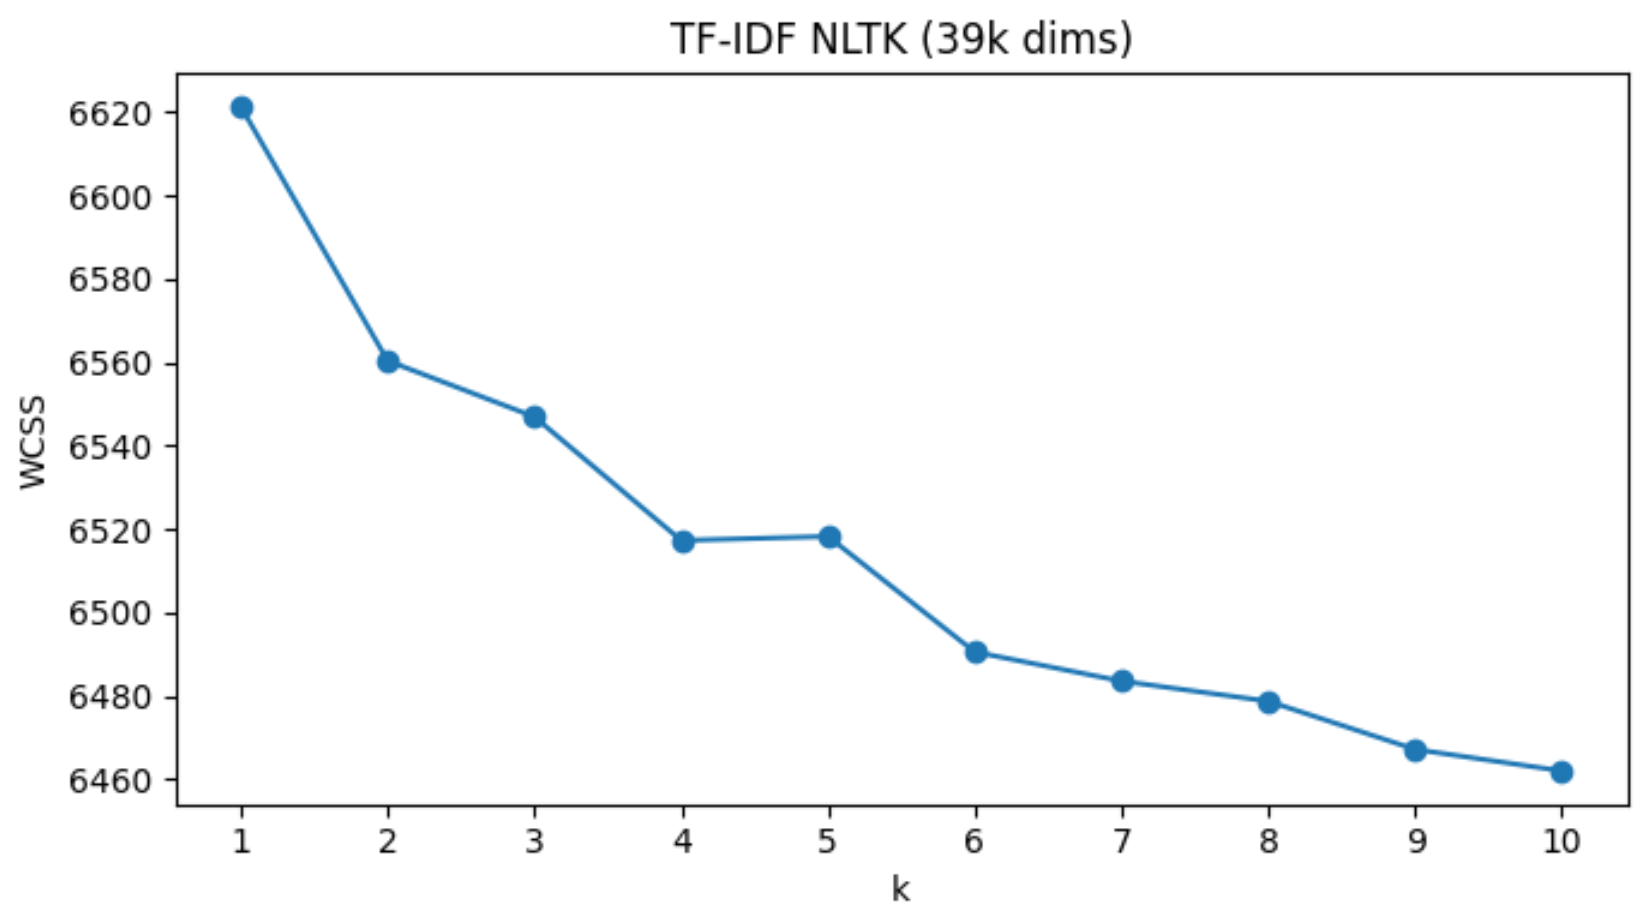
\includegraphics[width=\columnwidth]{tfidfcustomwcssvsk.png}
\caption{WCSS vs.\ $k$: Custom TF-IDF. Curve is nearly flat (about 2 to 3\% variation).}
\label{fig:elbow_custom}
\end{figure}

\begin{figure}[H]
\centering
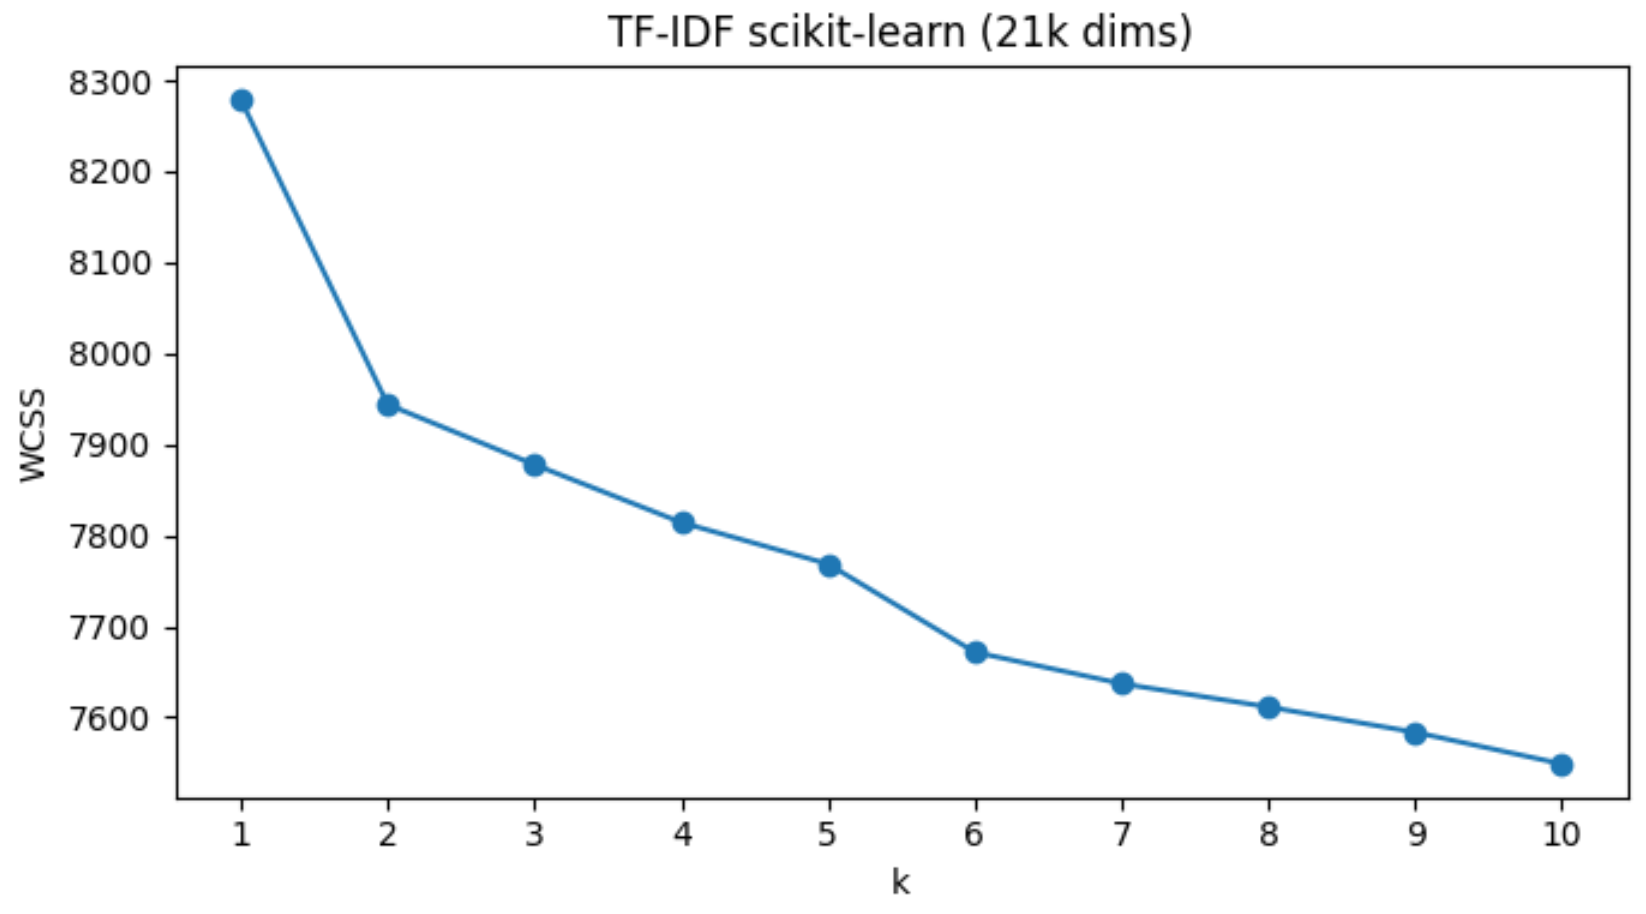
\includegraphics[width=\columnwidth]{tfidfsklearnwcssvsk.png}
\caption{WCSS vs.\ $k$: TF-IDF sklearn. Curve is nearly flat.}
\label{fig:elbow_sklearn}
\end{figure}

\begin{figure}[H]
\centering
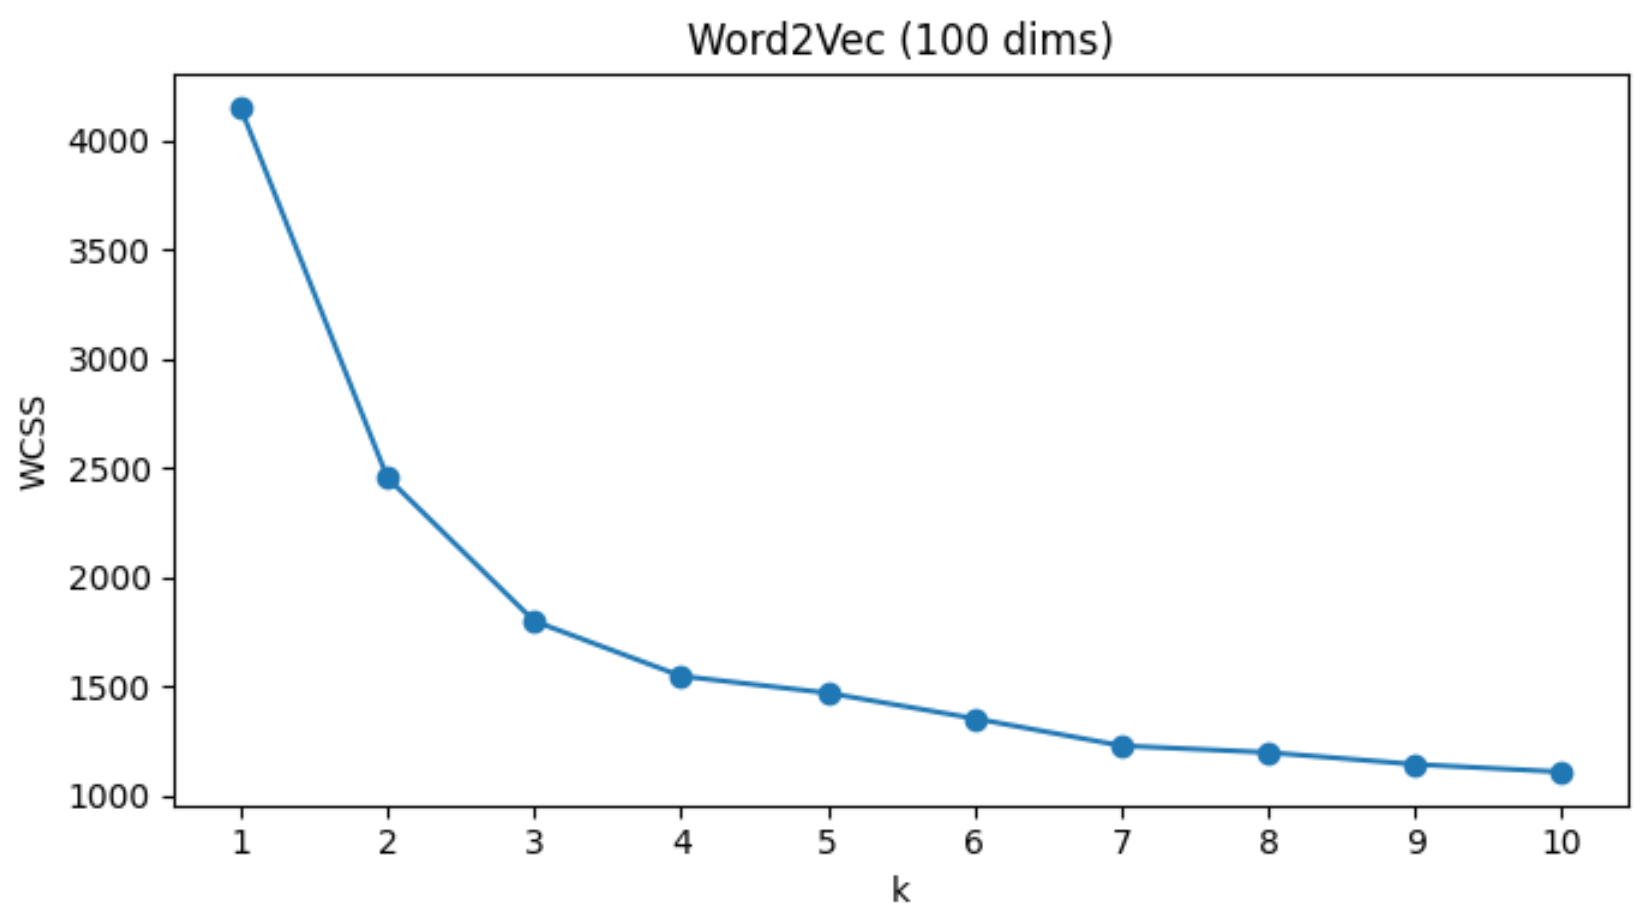
\includegraphics[width=\columnwidth]{word2vecwcssvsk.png}
\caption{WCSS vs.\ $k$: Word2Vec. Clear elbow at $k = 4$ to $5$.}
\label{fig:elbow_w2v}
\end{figure}

TF-IDF: curves almost flat, WCSS barely changes with $k$. In 20k to 39k \textit{sparse} dimensions K-Means does not separate clusters well. \textbf{Word2Vec} has a clear elbow: WCSS 4,148 ($k\!=\!1$) down to 1,547 ($k\!=\!4$), then flat; about 4 to 5 groups. We set $k = 6$ for the rest.

\subsection{Test Set Evaluation}

Table~\ref{tab:eval}: baseline (no SVD) vs SVD=300.

\begin{table*}[t]
\centering
\begin{tabular}{llrrrr}
\toprule
\textbf{Experiment} & \textbf{Embedding} & \textbf{Dims} & \textbf{WCSS} & \textbf{Silhouette} & \textbf{Davies-Bouldin} \\
\midrule
Baseline & Custom TF-IDF  & 39,204 & 907.04   & $-0.0652$ & 8.0253 \\
Baseline & TF-IDF sklearn & 21,519 & 1,897.93 & 0.0202    & 6.5651 \\
Baseline & Word2Vec       & 100    & 327.81   & 0.2986    & 1.3788 \\
\midrule
SVD=300  & Custom TF-IDF  & 300    & 284.70   & 0.0396    & 3.7895 \\
SVD=300  & TF-IDF sklearn & 300    & 656.30   & 0.0427    & 3.8062 \\
- & Word2Vec       & 100    & 322.24   & 0.3106    & 1.3923 \\
\bottomrule
\end{tabular}
\caption{Test set evaluation ($k = 6$, cosine distance, 5 repeats).
Silhouette ranges from $-1$ to $1$ (higher is better).
Davies-Bouldin: lower is better.}
\label{tab:eval}
\end{table*}

\begin{figure}[H]
\centering
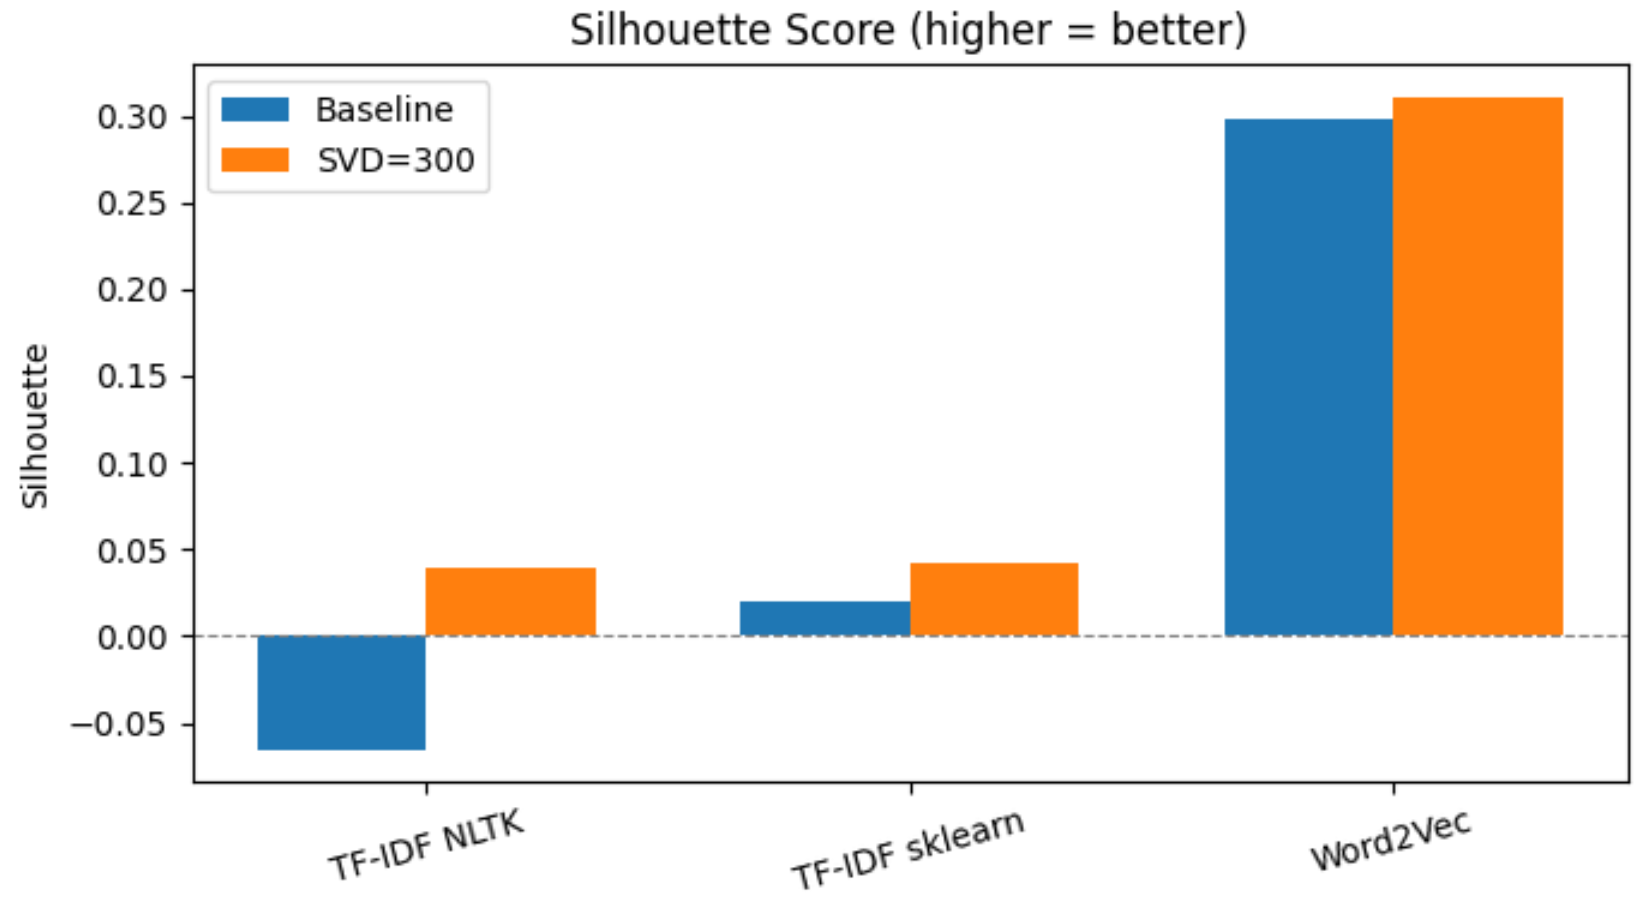
\includegraphics[width=\columnwidth]{silhouette.png}
\caption{Silhouette score: baseline vs.\ SVD=300 across embeddings.}
\label{fig:sil}
\end{figure}

\begin{figure}[H]
\centering
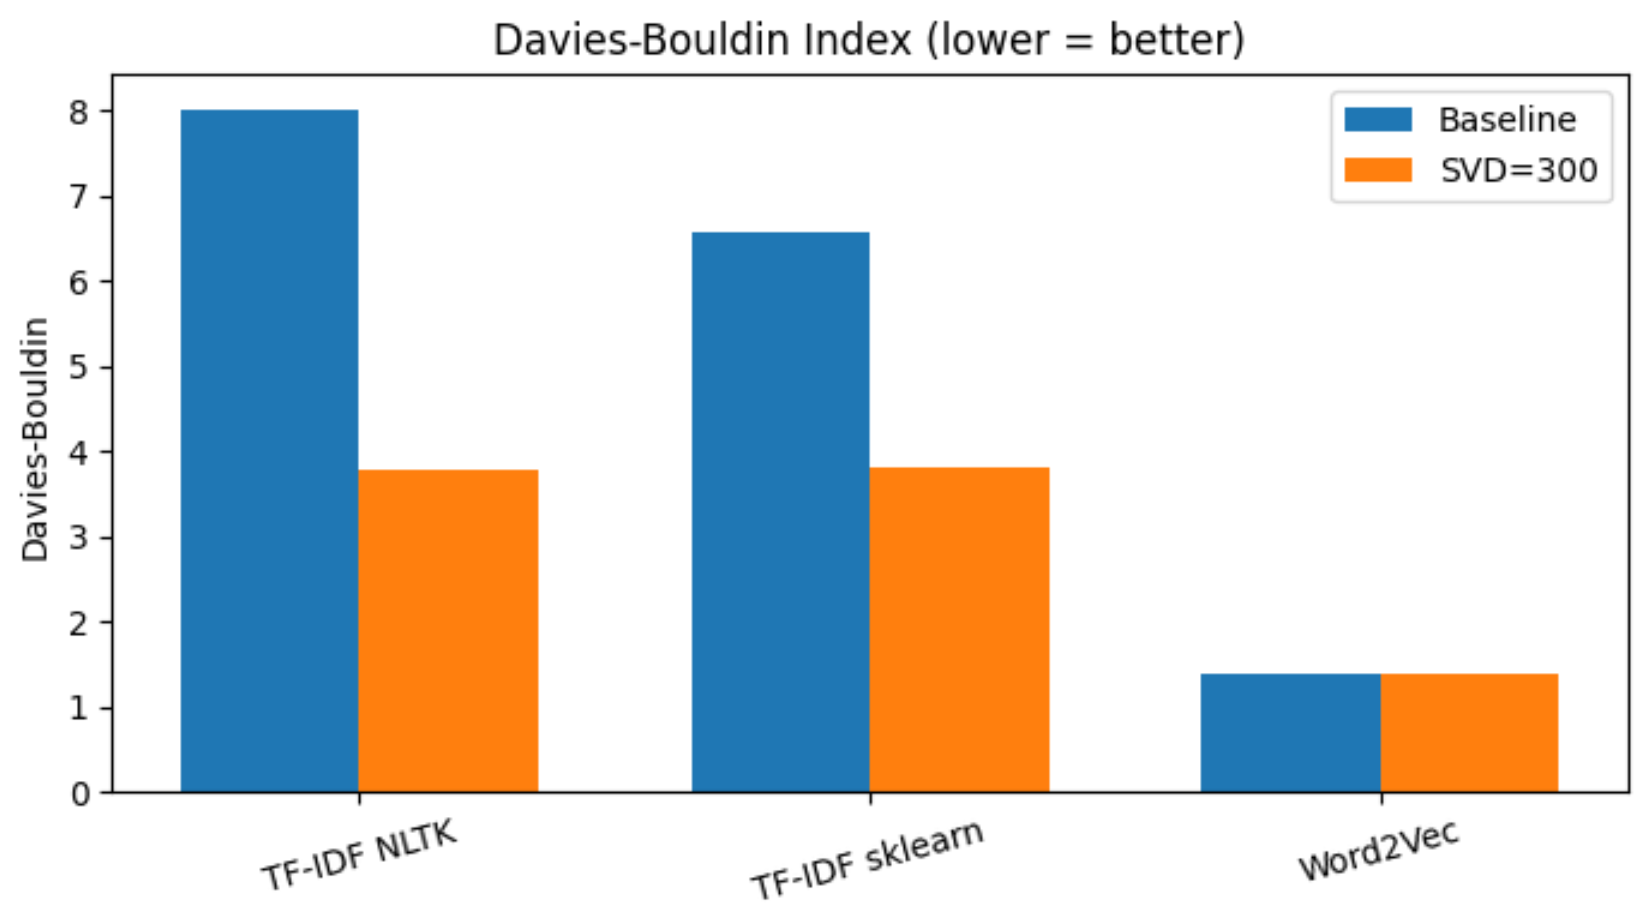
\includegraphics[width=\columnwidth]{daviesbouldinindex.png}
\caption{Davies-Bouldin index: baseline vs.\ SVD=300 across embeddings.}
\label{fig:db}
\end{figure}

\textbf{Word2Vec}: Silhouette 0.31, Davies-Bouldin 1.39. Raw TF-IDF: Silhouette $\approx 0$ (\textit{near-random}). With SVD, TF-IDF improves (Silhouette about $+0.04$, Davies-Bouldin about halved) but stays well below Word2Vec.

\subsection{Cluster Visualization}

t-SNE of the test set, points colored by cluster (Figures~\ref{fig:tsne_custom} to \ref{fig:tsne_w2v}).

\begin{figure}[H]
\centering
\includegraphics[width=\columnwidth]{"tsne tfidf custom.png"}
\caption{t-SNE projection: Custom TF-IDF (SVD=300), $k = 6$. Heavy overlap.}
\label{fig:tsne_custom}
\end{figure}

\begin{figure}[H]
\centering
\includegraphics[width=\columnwidth]{"tsne tfidf sklearn.png"}
\caption{t-SNE projection: TF-IDF sklearn (SVD=300), $k = 6$. Overlap; sklearn variant better than custom.}
\label{fig:tsne_sklearn}
\end{figure}

\begin{figure}[H]
\centering
\includegraphics[width=\columnwidth]{"tsne word2vec.png"}
\caption{t-SNE projection: Word2Vec, $k = 6$. Clearly separated clusters.}
\label{fig:tsne_w2v}
\end{figure}

\textbf{Word2Vec}: \textit{spatially distinct} blobs, little overlap. The two TF-IDF plots are \textit{interleaved}, boundaries unclear.

% =================================================================
\section{Conclusions}
% =================================================================

\begin{enumerate}
    \item \textbf{Embedding.} \textit{Word2Vec} (Silhouette 0.31) clearly beats both TF-IDF variants ($\leq 0.04$), with or without SVD.

    \item \textbf{SVD for TF-IDF.} In 20k to 39k \textit{sparse} dimensions, \textit{distance concentration} gives \textit{near-random} assignments. SVD to 300 dims roughly halves \textit{Davies-Bouldin} but does not match Word2Vec.

    \item \textbf{Preprocessing flags.} Tokenization, stopwords, stemming, SVD as separate flags allow ablation. CSV between preprocessing and clustering avoids re-running embeddings.

    \item \textbf{Limitations.} Reuters is \textit{multi-label}, K-Means is \textit{hard partitioning}; the two do not align. Word2Vec was not tuned. \textbf{HDBSCAN} or \textbf{LDA} may fit this setting better.
    Also, trying different kinds of embeddings (e.g. \textbf{GloVe} or \textbf{BERT}) could be a future possible test.
    
\end{enumerate}

\end{document}
